% Chapter 2
 % For referencing the chapter elsewhere, use \ref{Chapter1}
%\begin{figure}
\chapter{Document Extraction} % Main chapter title
\label{Chapter2}
%----------------------------------------------------------------------------------------

\section{Flow Chart}
\nopagebreak
% Define block styles
\tikzset{
	desicion/.style={
		diamond,
		draw,
		text width=6em,
		text badly centered,
		inner sep=0pt
	},
	block/.style={
		rectangle,
		draw,
		text width=15em,
		text centered,
		rounded corners
	},
	cloud/.style={
		draw,
		ellipse,
		minimum height=1em
	},
	descr/.style={
		fill=white,
		inner sep=2.5pt
	},
	connector/.style={
		-latex,
		font=\scriptsize
	},
	rectangle connector/.style={
		connector,
		to path={(\tikztostart) -- ++(#1,0pt) \tikztonodes |- (\tikztotarget) },
		pos=0.5
	},
	rectangle connector/.default=-2cm,
	straight connector/.style={
		connector,
		to path=--(\tikztotarget) \tikztonodes
	}
}
\begin{center}
	\begin{figure}[hbt]
		\centering
	\begin{tikzpicture}
\matrix (m)[matrix of nodes, column  sep=2cm,row  sep=8mm, align=center, nodes={rectangle,draw, anchor=center} ]{
	|[block]| {Start}              &  \\
	|[block]| { Capture the image \\ of the document }               &                                            \\
	|[desicion]| {Image greater than 640 X 480 ?}          & |[block]| {Resize image by the scale factor based on the ratio between the size of the image and 640 X 480}                                               \\
	|[block]| {Convert to grayscale and enhance image by \\ Sharpening, Bilateral Filtering}    &                                             \\
	|[block]| {Canny Edge Detection}    &            |[block]| {Stop}                                   \\
	|[block]| {Fill small holes by Erosion/Dilation}    &    |[block]| {Do adaptive thresholding to create a binary image}                                          \\
	|[block]| {Extract biggest rectangular \\ convex contour}        &       |[block]| {Warp the image using the perspective transform and do bilinear interpolation}                                      \\
	|[block]| {Extract corners using \\ Harris Corner Detector and order the corners in clockwise direction}    &   |[block]| {Upscale corners to original size and extract perspective \\transform between this \\ polygon and an ideal rectangle }                                         \\
};
\path [>=latex,->] (m-1-1) edge (m-2-1);
\path [>=latex,->] (m-2-1) edge (m-3-1);
\path [>=latex,->] (m-3-1) edge node[auto] {\scriptsize{NO}} (m-4-1);
\path [>=latex,->] (m-3-1) edge node[auto] {\scriptsize{YES}} (m-3-2);
\draw [>=latex,->] (m-3-2) |- (m-4-1);
\path [>=latex,->] (m-4-1) edge (m-5-1);
\path [>=latex,->] (m-5-1) edge (m-6-1);
\path [>=latex,->] (m-6-1) edge (m-7-1);
\path [>=latex,->] (m-7-1) edge (m-8-1);
\path [>=latex,->] (m-8-1) edge (m-8-2);
\path [>=latex,->] (m-8-2) edge (m-7-2);
\path [>=latex,->] (m-7-2) edge (m-6-2);
\path [>=latex,->] (m-6-2) edge (m-5-2);

\end{tikzpicture}
    \caption{Flow Chart for Document Extraction}
\label{fig:DocumentExtractionFlowChart}
\end{figure}
\end{center}
%\caption[Document Extraction]{Flowchart for Document Extraction.}


%\end{figure}

\section{Document Extraction Techniques}

Consider the image shown below from which the document is to be extracted. 
\\ \\

\begin{figure}[th]
	\centering
	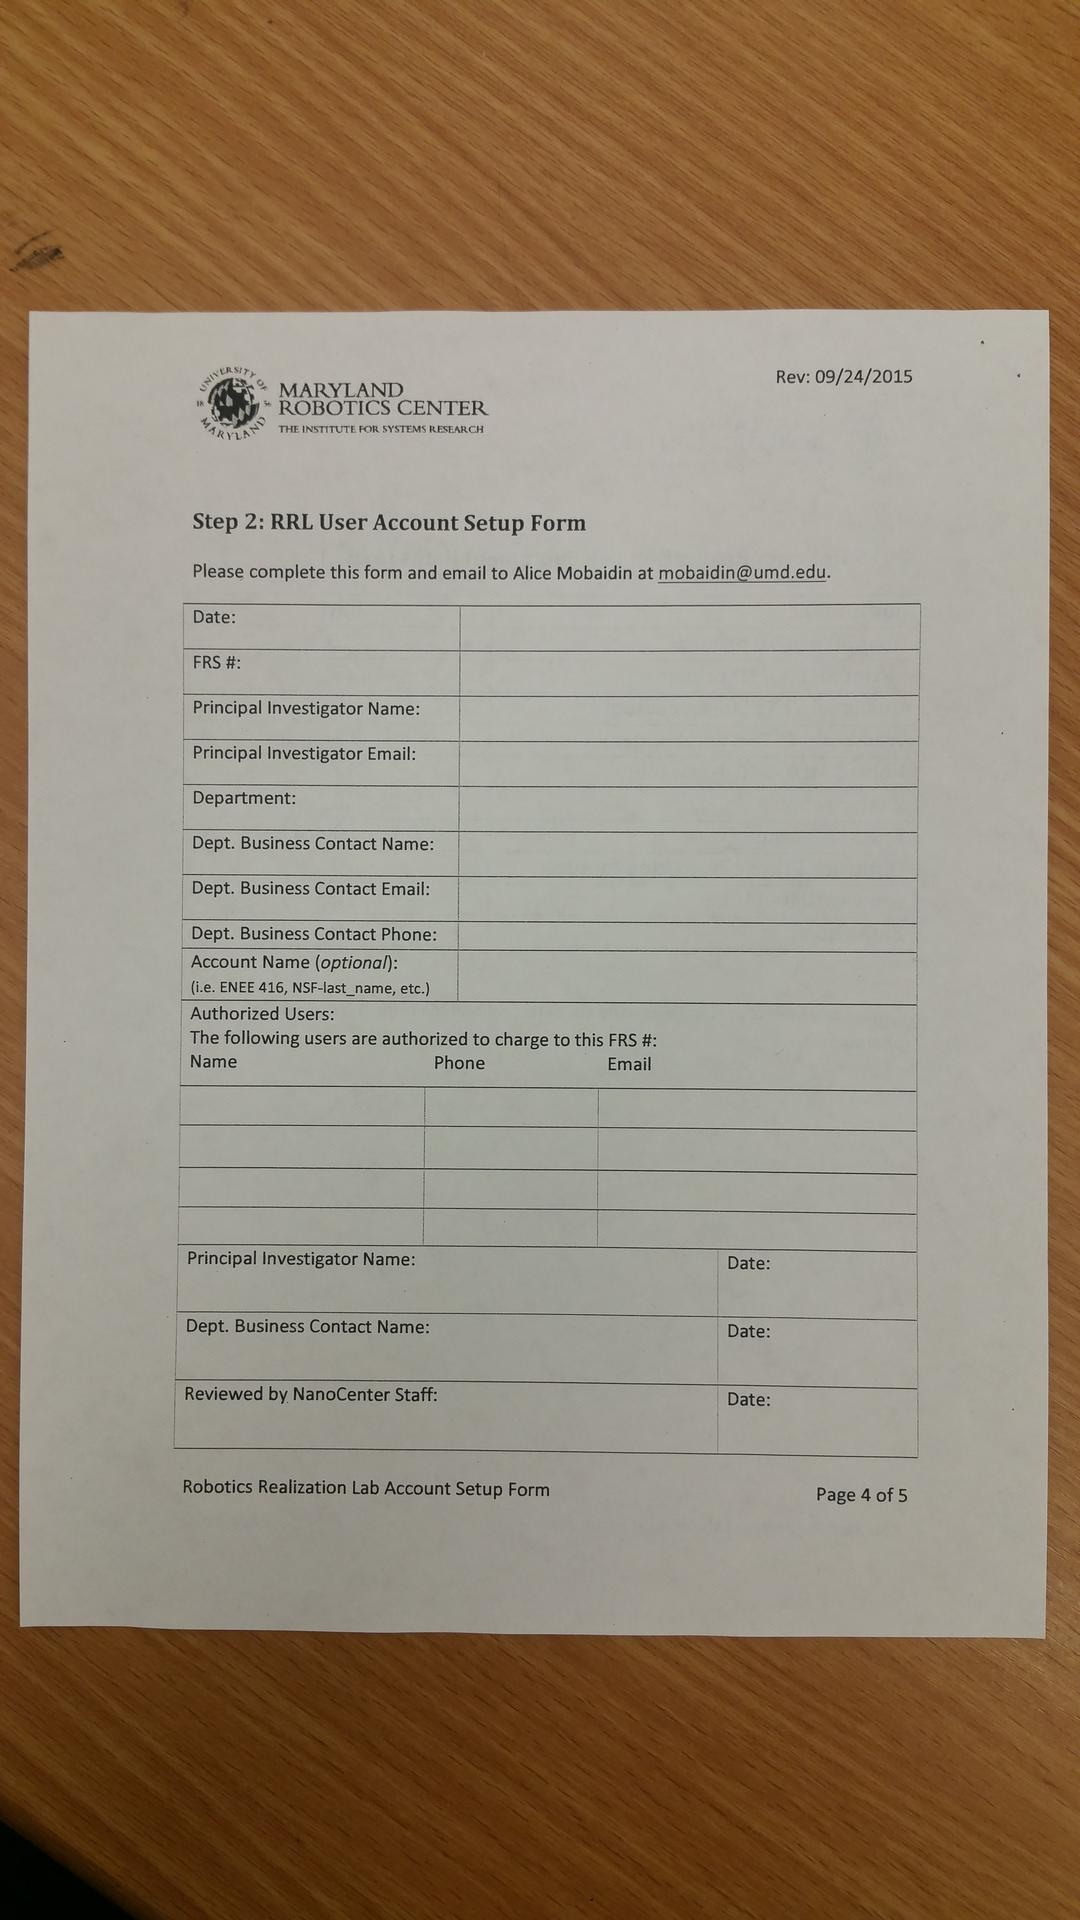
\includegraphics[height=18cm ]{Figures/resized_input}
	%	\decoRule
	\caption[Reference Image]{Reference Image.}
	\label{fig:ReferenceImage}
\end{figure}

\pagebreak
All the techniques involved in extracting the document/sheet from the given image are briefly explained below. \\

\subsection{Image Enhancement}

The input RGB image is resized to be below 640 X 480 pixels, if the image size is greater than that. Then the resized image is converted to grayscale by doing weighted addition of R, G and B components and normalizing them to fit 0 to 255 scale. Then the image is sharpened in-order to boost its edges. The edges can be \keyword{sharpened} by adding a portion of the high pass filtered image to the original image. In order to smoothen out any noise in the image, \keyword{bilateral filter} (\cite{Reference17}) is used. The bilinear filter implemented as a part of this project uses a kernel size of 5 with gaussian weight of 25 and range weight of 15 . The bilateral filter basically does gaussian filtering everywhere in the image except at the edges. \\ \\
 The resulting enhanced image is shown below. \\


\begin{figure}[th]
	\centering
	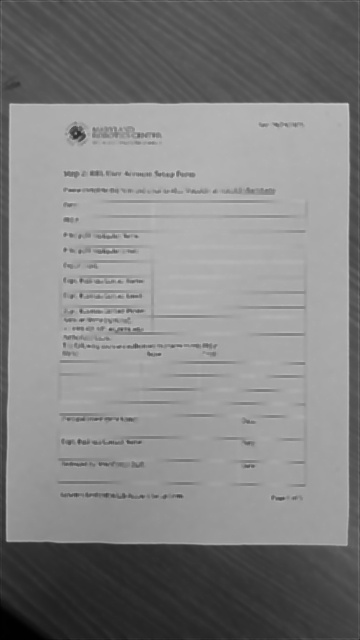
\includegraphics[height=15cm ]{Figures/image_enhancement}
%	\decoRule
	\caption[Image Enhancement]{Image Enhancement.}
	\label{fig:ImageEnhancement}
\end{figure}

\subsection{Canny Edge Detection}

The edges from the enhanced image can be extracted using the \keyword{Canny Edge Detection} method (\cite{Reference7} ). 
\\
\\
The canny edge detection algorithm proceeds as shown in the flow chart below.
\\
\\
	\begin{center}
	\begin{figure}[hbt]
	\centering
	\begin{tikzpicture}
	\matrix (m)[matrix of nodes, column  sep=0cm,row  sep=8mm, align=center, nodes={rectangle,draw, anchor=center} ]{
		|[block]| {Start}              &  \\
		|[block]| {Input Image}              &  \\
		|[block]| { Gaussian Blur }               &                                            \\
		|[block]| {Sobel Filter}          &             \\
		|[block]| {Non Maximum Suppression}    &                                             \\
		|[block]| {Double Thresholding}    &         \\
		|[block]| {Hysterisis}    &                   \\
		|[block]| {Edges}        &             \\
		|[block]| {Stop}        &             \\
	};
	\path [>=latex,->] (m-1-1) edge (m-2-1);
	\path [>=latex,->] (m-2-1) edge (m-3-1);
	\path [>=latex,->] (m-3-1) edge (m-4-1);
	\path [>=latex,->] (m-4-1) edge (m-5-1);
	\path [>=latex,->] (m-5-1) edge (m-6-1);
	\path [>=latex,->] (m-6-1) edge (m-7-1);
	\path [>=latex,->] (m-7-1) edge (m-8-1);
	\path [>=latex,->] (m-8-1) edge (m-9-1);

	\end{tikzpicture}

	\caption{Flow Chart for Canny Edge Detection}
`   \label{fig:CannyEdgeDetectionFlowChart}

\end{figure}
\end{center}


This is a multi-step edge detection algorithm that typically uses and optimizes other edge detection operators such as Prewitt, Robert and Sobel. First the input image is smoothened with a \keyword{Gaussian Filter}. Then an edge detection operator like \keyword{Sobel Filter} is applied to the image and the intensity gradient and direction is computed. Based on the gradient and its direction, \keyword{non maximum suppression} is applied to make the edges thinner. Strong and weak edges from the resulting image are identified by \keyword{double thresholding} it. The weak edges are then tracked to see if its connected to other strong edges, in which case the weak edge will now be considered as strong edge or will be eliminated otherwise. This process is called \keyword{hysterisis}.

\pagebreak

The result of canny edge detection on the previously enhance image is shown below. \\ \\

\begin{figure}[th]
	\centering
	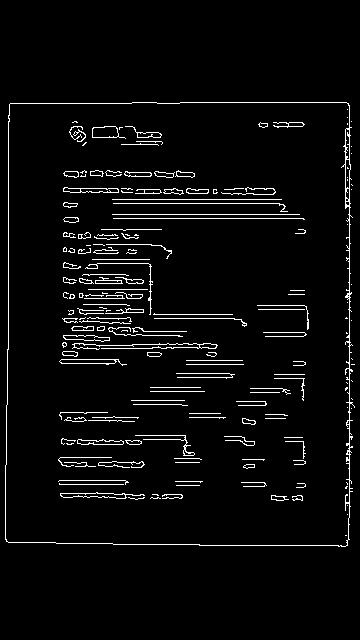
\includegraphics[height=18cm ]{Figures/canny_edge_detection}
	%	\decoRule
	\caption[Canny Edge Detection]{Canny Edge Detection.}
	\label{fig:CannyEdgeDetection}
\end{figure}
\pagebreak
\subsection{Morphological Operations}

The edges extracted from the enhanced image can sometimes have some discontinuities and minute holes that might need to be eliminated for further processing to work. In order to do that, a variety of morphological operations,namely \keyword{Erosion} and \keyword{Dilation}, are used. Dilation replaces the pixel in an image with the pixel that has the highest value. Hence, this operation thickens the white edges. Erosion on the other hand replaces the pixel in an image with the pixel that has the lowest value. Thus, this operation thins the white edges. A combination of these two operations can be used to do morphological opening and closing. The edges are first dilated and then eroded in order to close the discontinuities. This combination is referred to as \keyword{ morphological closing}. Then the edges are eroded and dilated in order to make the edges thinner. This combination is referred to as \keyword{morphological opening}.
\\
\\
The result of morphological closing and opening on the extracted edges are shown below.\\ 

\begin{figure}[th]
	\centering
	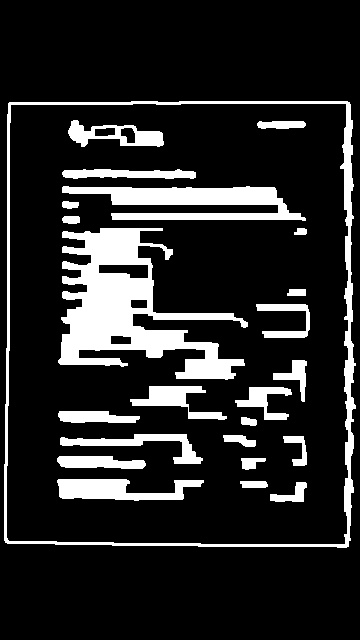
\includegraphics[height=16cm ]{Figures/morphological_operation}
	%	\decoRule
	\caption[Morphological Operations]{Morphological Operations.}
	\label{fig:MorphologicalOperations}
\end{figure}

\pagebreak

\subsection{Contour Detection}

The image computed previously contains a lot of \keyword{contours}. The contours from this image are extracted using OpenCV's (\cite{Reference1}) \keyword{'findContour'} function . Contours are estimated by using the \keyword{Boundary Following Algorithm for Topological Analysis}, proposed by \cite{Reference4}. The largest convex contour, with 4 vertices, is found and the pixels inside this contour is assumed to contain the document that has to be scanned .
\\
\\
The estimated contour is overlaid on the original image and shown below.\\ 

\begin{figure}[th]
	\centering
	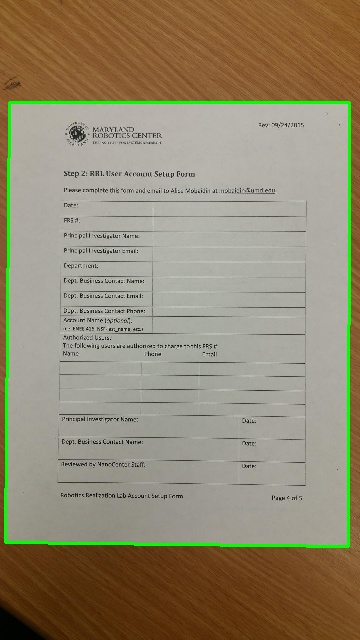
\includegraphics[height=16cm ]{Figures/contour_detection}
	%	\decoRule
	\caption[Contour Detection]{Contour Detection.}
	\label{fig:ContourDetection}
\end{figure}

\pagebreak

\subsection{Harris Corner Detection}

The contour estimated above basically has 4 corners. In order to compute them \keyword{Harris Corner Detection} (\cite{Reference6}) is used. 
\\
\\
The Harris Corner Detection algorithm proceeds as shown in the flow chart below.
\\
\\
\begin{center}
	\begin{figure}[hbt]
		\centering
		\begin{tikzpicture}
		\matrix (m)[matrix of nodes, column  sep=0cm,row  sep=8mm, align=center, nodes={rectangle,draw, anchor=center} ]{
			|[block]| {Start}              &  \\
			|[block]| {Estimated Contour}              &  \\
			|[block]| {Sobel Filter}          &             \\
			|[block]| {Compute Harris Matrix 
					   \[
					   M =\Sigma_{x,y}w(x,y)
					   \begin{bmatrix}
					   I_{x}^{2} & I_{x}I_{y}  \\
					   I_{x}I_{y} & I_{y}^{2} 
					   \end{bmatrix}
					   \]}          &             \\
			|[block]| {Compute Harris Response
					$ R= |M| -k.Trace(M^{2}) $}    &                                             \\
			|[block]| {Adaptive Thresholding}    &         \\
			|[block]| {Non Maxima Suppression}        &             \\
			|[block]| {Corners}        &             \\
			|[block]| {Stop}        &             \\
		};
		\path [>=latex,->] (m-1-1) edge (m-2-1);
		\path [>=latex,->] (m-2-1) edge (m-3-1);
		\path [>=latex,->] (m-3-1) edge (m-4-1);
		\path [>=latex,->] (m-4-1) edge (m-5-1);
		\path [>=latex,->] (m-5-1) edge (m-6-1);
		\path [>=latex,->] (m-6-1) edge (m-7-1);
		\path [>=latex,->] (m-7-1) edge (m-8-1);
		\path [>=latex,->] (m-8-1) edge (m-9-1);
		
		\end{tikzpicture}
		
		\caption{Flow Chart for Harris Corner Detection}
		`   \label{fig:HarrisCornerDetectionFlowChart}
		
	\end{figure}
\end{center}

Harris Corner Detection method estimates the location of corners based on the gradients at each pixel. It fundamentally relies on the property that corners have large gradients in both x and y direction. The algorithm proceeds by computing the x and y gradients of the image using operators like Sobel. Based on these gradients, the Harris Matrix is computed. Then the Harris Response is obtained from the Harris Matrix M where k's best estimate by Harris was found to be 0.04. The response image is adaptively thresholded in order to obtain the corners. There might be a lot of estimated corners very close to each other , these group of corners are replaced by just one corner by doing non-maxima suppression. 

\pagebreak

The result of harris corner detection on the estimated contour is overlaid on the original image shown below \\ \\

\begin{figure}[th]
	\centering
	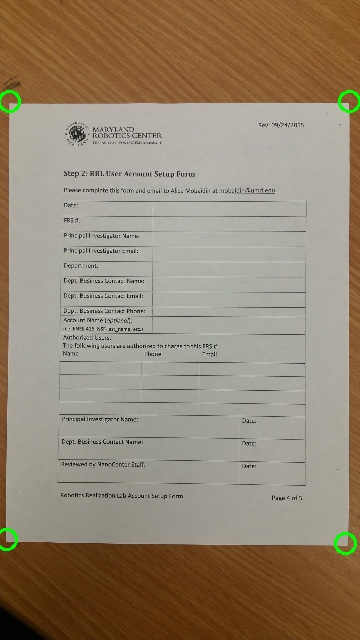
\includegraphics[height=18cm ]{Figures/corner_detection}
	%	\decoRule
	\caption[Corner Detection]{Corner Detection.}
	\label{fig:CornerDetection}
\end{figure}

\pagebreak

\subsection{Perspective Transform and Warping}

The four corners obtained above are ordered in the clockwise manner. The width and height of the contour are approximated based on the location of these corners and then a reference rectangle is constructed based on this. 
\\
\\
The \keyword{perspective transform} (\cite{Reference16}) between the corners of the contour and the corners of the reference rectangle can be computed to warp the image as shown below. \\

\begin{center}
		\centering
	\begin{figure}[hbt]
		\centering
		\begin{tikzpicture}
		\matrix (m)[matrix of nodes, column  sep=1cm,row  sep=7mm, align=center, nodes={rectangle,draw, anchor=center} ]{
			|[block]| {Start}              &  \\
			|[block]| {Corners}              &  \\
			|[block]| {Order Clockwise}          &             \\
			|[block]| {Solve the following for 4 corners 
				\[
				\begin{bmatrix}
				x_{1} & x_{2} & x_{3}  \\
				y_{1} & y_{2} & y_{3} \\
				1 & 1 & 1
				\end{bmatrix}.\begin{bmatrix}
				\lambda  \\
				\mu \\
				\tau
				\end{bmatrix} = \begin{bmatrix}
				x_{4}  \\
				y_{4} \\
				1
				\end{bmatrix}
				\]}          &             \\
			|[block]| {Scale columns by \\ computed coefficients
								\[ A = 
				\begin{bmatrix}
			\lambda.x_{1} & \mu .x_{2} & \tau .x_{3}  \\
			\lambda	.y_{1} & \mu .y_{2} & \tau .y_{3} \\
			\lambda & \mu & \tau
				\end{bmatrix}\]}    &                    \\
			|[block]| {Repeat previous 2 steps for reference rectangle to get B}    &  |[block]| {Stop}                                 \\
			|[block]| {Compute Perspective Transform\\ $ C = B.A^{-1}  $}        &     	|[block]| {Do Bilinear Interpolation}            \\
			|[block]| { Get homogeneous co-ordinates of transformed points\[ \begin{bmatrix}
				x^{'}  \\
				y^{'} \\
				z^{'}
				\end{bmatrix} = C. \begin{bmatrix}
				x  \\
				y \\
				z
				\end{bmatrix}
				\]}        &            
			|[block]| {Warp Image by normalizing homogeneous co-ordinates \\ $ x^{''} = \dfrac{x^{'}}{z^{'}} \ ,\  y^{''} = \dfrac{y^{'}}{z^{'}} $}        &             \\
		};
		\path [>=latex,->] (m-1-1) edge (m-2-1);
		\path [>=latex,->] (m-2-1) edge (m-3-1);
		\path [>=latex,->] (m-3-1) edge (m-4-1);
		\path [>=latex,->] (m-4-1) edge (m-5-1);
		\path [>=latex,->] (m-5-1) edge (m-6-1);
		\path [>=latex,->] (m-6-1) edge (m-7-1);
		\path [>=latex,->] (m-7-1) edge (m-8-1);
		\path [>=latex,->] (m-8-1) edge (m-8-2);
		\path [>=latex,->] (m-8-2) edge (m-7-2);
		\path [>=latex,->] (m-7-2) edge (m-6-2);
		\end{tikzpicture}
		\caption{Flow Chart for Computing Perspective Transform}
		`   \label{fig:PerspectiveTransformComputation}
	\end{figure}
\end{center}

\pagebreak

The result of \keyword{warping} the image using the computed perspective transform and doing \keyword{bilinear interpolation} is shown below\\ \\

\begin{figure}[th]
	\centering
	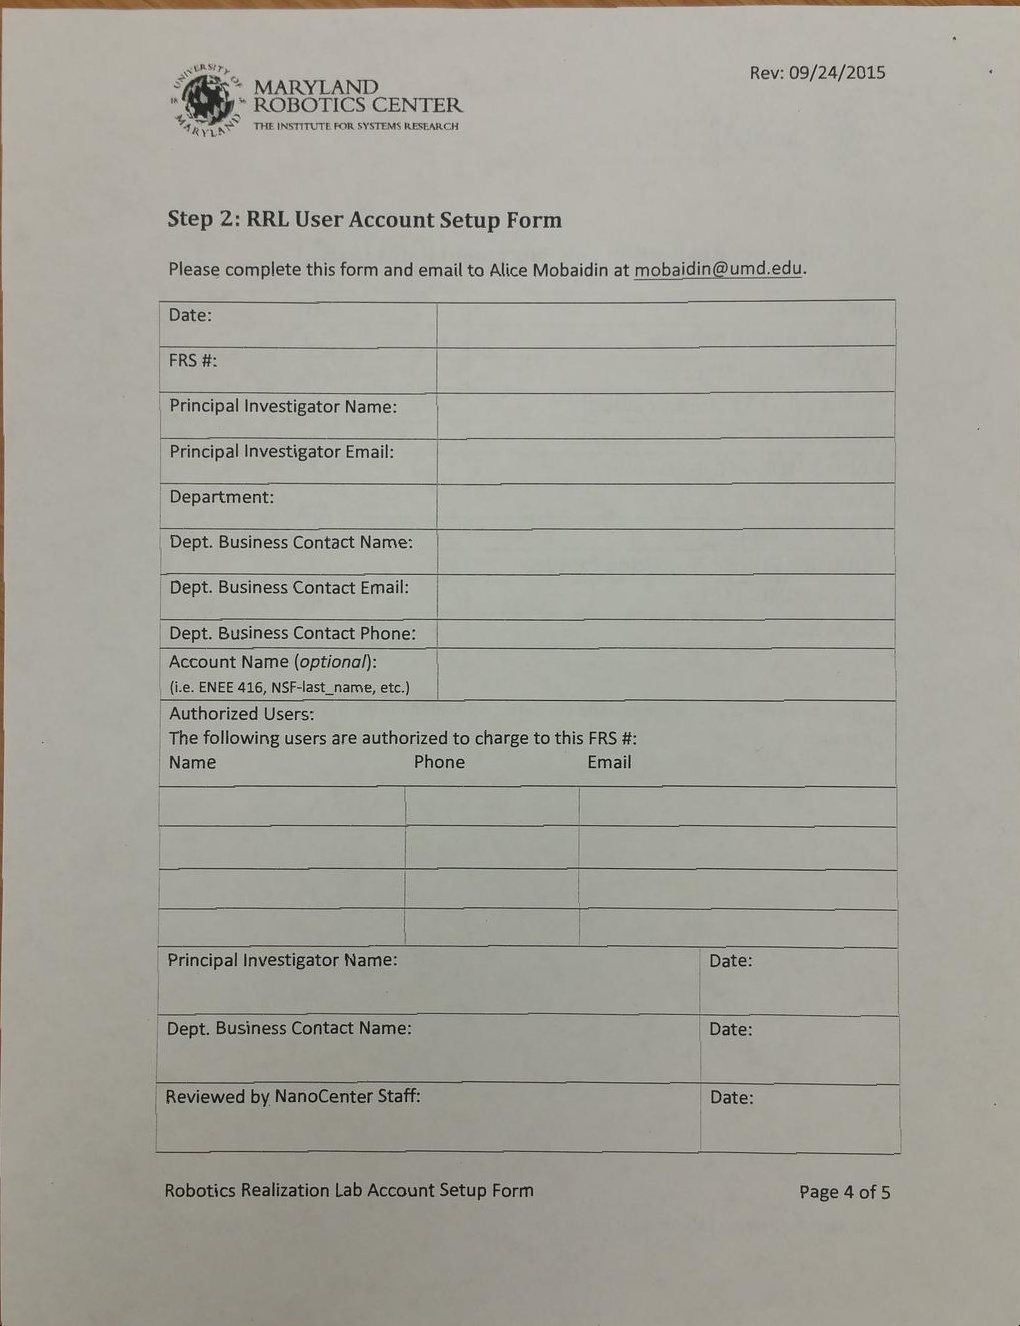
\includegraphics[height=18cm ]{Figures/warped_image}
	%	\decoRule
	\caption[Warped Reference Image]{Warped Reference image.}
	\label{fig:WarpedReferenceImage}
\end{figure}

\pagebreak

\subsection{Adaptive Thresholding}

The warped RGB image can be converted to binary Black/White format, suitable for printing/registration purposes, by doing \keyword{Adaptive Thresholding} (\cite{Reference10}) . This is a data dependent thresholding technique. It's fundamental principle is that the region of interest can be segmented out by using the blurred version of an image minus a constant as the threshold. Different types of filters like Mean filters, Gaussian filter , Median filter can be used to blur the image. Here the Gaussian Minus C algorithm is used. C was experimentally determined to be 5. This would be really useful for \keyword{text segmentation} (\cite{Reference14}) \. \\ \\ The adaptively thresholded reference image is shown below. \\

\begin{figure}[th]
	\centering
	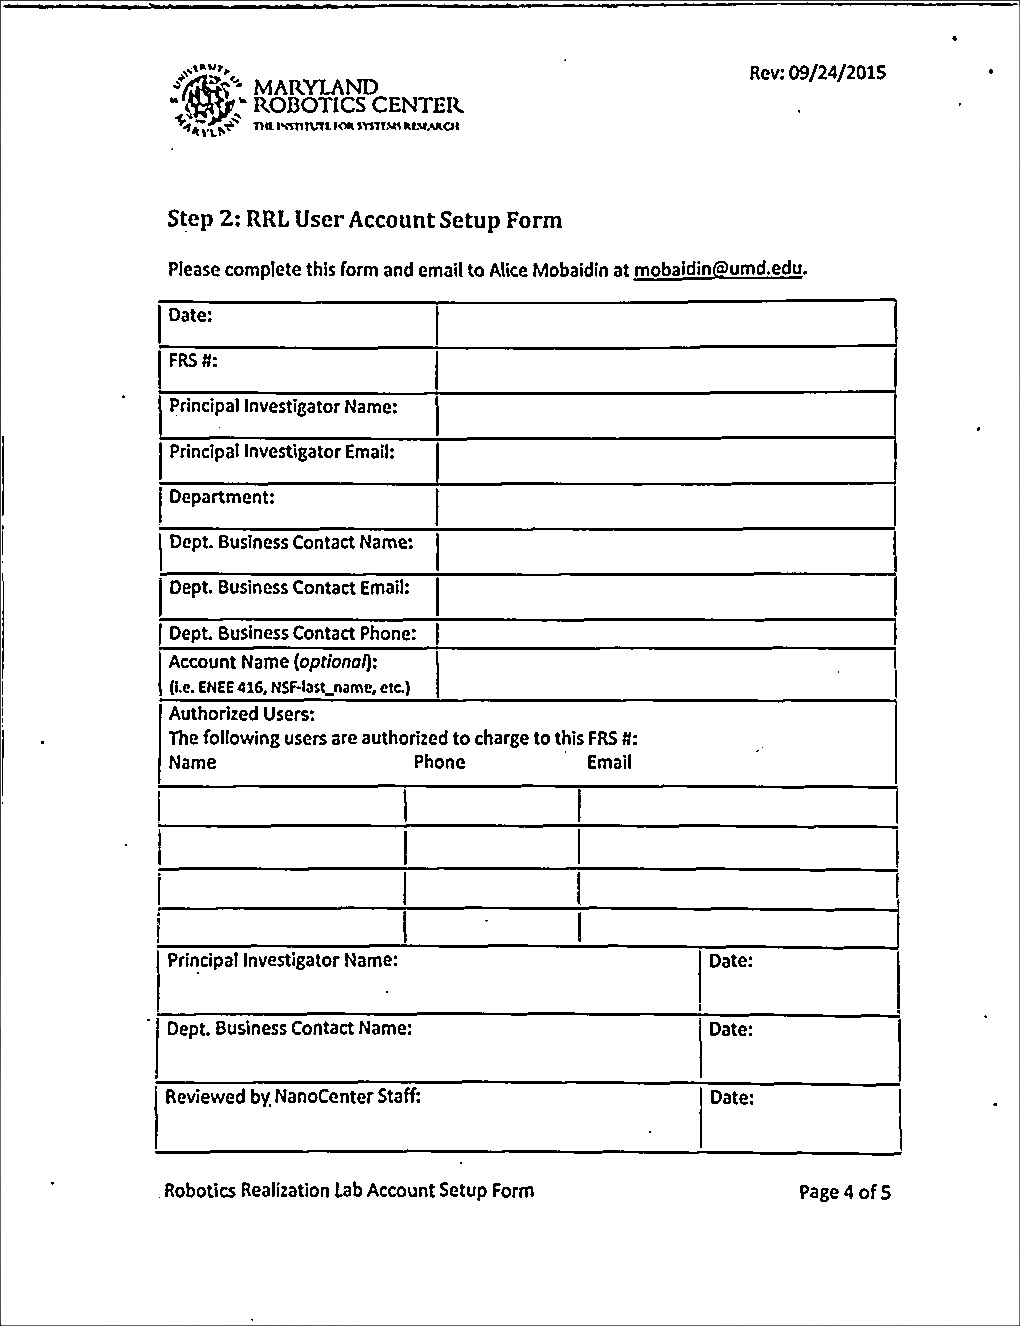
\includegraphics[height=17cm ]{Figures/adaptive_thresholding}
	%	\decoRule
	\caption[AdaptiveThresholding]{Adaptive Thresholding.}
	\label{fig:AdaptiveThresholding}
\end{figure}




%----------------------------------------------------------------------------------------


